\documentclass[12pt,a4paper]{article}
\usepackage{amsmath}
\usepackage{amsfonts}
\usepackage{amssymb}
\usepackage{graphicx}
\usepackage{secdot}
\usepackage[left=2cm,right=2cm,top=2cm,bottom=2cm]{geometry}

\author{ Shibayan Biswas, AE21B109\\ Department of Aerospace Engineering\\ IIT Madras\\[3ex] Instructor:\\ \large Professor Dr. Manikandan Mathur}

\title{Experiment- 6}

\date{September 28, 2022}

\begin{document}

\maketitle
\hline
\section{Aim:}
To calculate the Meta-centric Height experimentally and theoretically and check how closely the values match.
\section{Theory:}
In this section let us go through a brief introduction on the topics "Buoyancy", "Centre of Buoyancy", "Meta-centre" and "Meta-centric height" because concepts related to these topics are used for calculating the results from the observed data for the given experiment; which is present in the later sections of this document. 
\subsection{Buoyancy:}
Buoyancy or upthrust is a force that opposes the weight of a fully or partially submerged body. The magnitude of this force is directly proportional to the pressure difference, which in turn is equivalent to the weight of the fluid that would otherwise occupy the submerged volume of the object, i.e. the displaced fluid.\\
\\The magnitude of the buoyant force is given by the expression :
\begin{equation}
\text{$F_B$} = \text{$V_i \rho_l g$}
\end{equation}
where,
\begin{itemize}
\item $V_i$ is the volume displaced by the submerged or partially submerged body. In other words, it’s the immersed volume of the object.
\item $\rho_l$ is the density of the fluid in which the object is submerged.
\item g is the acceleration due to gravity.
\end{itemize}
\subsection{Centre of Buoyancy:}
The centre of gravity of the volume of displaced fluid when an object is immersed in the fluid is called the centre of buoyancy. A floating body, partially submerged in water may not have a coinciding centre of gravity and centre of buoyancy.\\
\\Hence we have a force equal to the weight of the body W acting on the centre of gravity vertically downwards and an equal force acting on the centre of buoyancy vertically upwards. Now, if we displace the body by an angle $\theta$ the centre of buoyancy shifts and the centre of buoyancy and the centre of gravity may not be along the same vertical line. This gives rise to the following cases:
\begin{itemize}
\item If B is above G, a restoring couple is always generated: Stable equilibrium.
\item If B is below G, there are three possibilities:
\begin{itemize}
\item If B is to the left of G, a restoring couple is generated: Stable equilibrium.
\item If B is to the right of G, an overturning couple is generated: Unstable equilibrium.
\item If B is along the vertical line passing through G, no moment is generated: Neutral equilibrium.
\end{itemize}
\end{itemize}
Therefore, to calculate the stability of a floating body, we define a term called the meta-centre.
\subsection{Meta-centre (M):}
In fluid dynamics, meta centre is the theoretical point where an imaginary vertical line passing through the centre of buoyancy and centre of gravity overlaps an unreal vertical line passing through a separate centre of buoyancy produced whenever the body is relocated, or tipped, throughout the water, however slightly.\\
\\As per the Meta-center definition, the centre of buoyancy of a ship goes laterally when it heels (rolls sideways). It may also rise or fall in relation to the water line. The meta-centre is the point where a vertical line via the heeled center of buoyancy intersects with the line via the existing, vertical centre of buoyancy. By description, the meta-centre stays exactly just above the centre of buoyancy.
\subsection{Meta-centric Height (GM):}
The metacentric height (GM) is a calculation of a floating body's initial static stability. The distance between that ship's centre of gravity and its metacentre is computed. Considerably greater stability against overturning is associated with a higher metacentric height.\\
\\The natural time of rolling of a hull is also influenced by metacentric height, with quite massive metacentric heights typically linked with shorter duration of roll, that are inconvenient for passengers. As a result, passenger ships should have a reasonably large metacentric height, but not overly so.\\
\\The condition of stable equilibrium for a floating body can be expressed in terms of meta-centric height as follows:
\begin{itemize}
\item $GM > 0$ (M is above G): Stable equilibrium
\item GM = 0 (M coinciding with G): Neutral equilibrium
\item $GM < 0$ (M is below G): Unstable equilibrium
\end{itemize}
Further in this report, we shall use the following formulae to calculate metacentric height.\\
\begin{figure}[!ht]
	\begin{center}
		\framebox{
			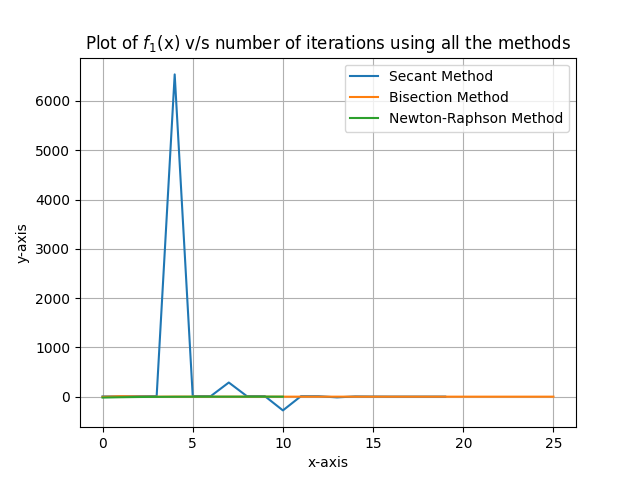
\includegraphics[scale=0.4]{Figure_7.png}
		}
	\end{center}
	\caption{Diagram of the setup}
\end{figure}\\
Theoretically we can determine the value of Meta-centric Height (GM) by the formula given below:
\begin{equation}
    \text{GM} = \text{$\frac{\text{$b^2$}}{\text{$12d$}}$} - \text{(y - $\frac{\text{$d$}}{\text{$2$}}$)}
\end{equation}
GM is the metacentric height.\\
b = 0.2 m is the pontoon width in the apparatus used.\\
$d = \frac{\text{W}}{\text{$lb\rho$}}$ = 18.64mm is the depth of immersion.\\
W = 1.305 kg is the total pontoon weight.\\
l = 0.35 m is the pontoon length in the apparatus used.\\
$\rho$ = 1000 $\frac{\text{$Kg$}}{\text{$m^3$}}$ is the density of water.\\
\\Experimentally we can determine the value of Meta-centric Height (GM) by the formula given below:
\begin{equation}
    \text{GM} = \text{$\frac{\text{$Px$}}{\text{$W tan\theta$}}$}
\end{equation}
GM is the metacentric height.\\
P = 0.305kg is the inclining weight only.\\
x = distance of inclining weight from centre line of pontoon.\\
W = 1.305kg is the total pontoon weight.\\
$\theta$ = Angle of heel.
\section{Experimental Apparatus:}
To determine the metacentric height, the following Apparatus is used:
\begin{itemize}
\item Metacentric height apparatus.
\item Hydraulics bench.
\item Water.
\end{itemize}
The following figure shows the metacentric height apparatus.\\
It consists of a rectangular plastic pontoon with a vertical mast, horizontal rod and a calibrated scale to read the linear displacement as well as angle in degrees.\\
There is a movable weight on the vertical mast and another on the horizontal rod adjacent to the scale.\\
Suspended from the vertical mast is a plumb bob used to read the angle in degrees.
\begin{figure}[!ht]
	\begin{center}
			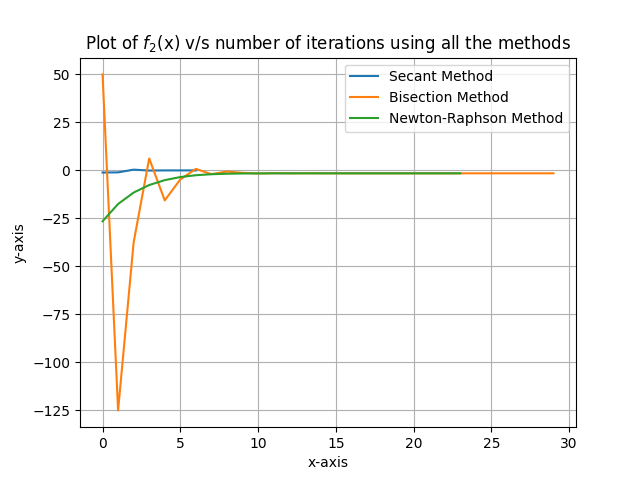
\includegraphics[scale=0.5]{Figure_8.png}
	\end{center}
	\caption{Meta-centric height apparatus setup}
\end{figure}
\section{Procedure:}
To determine the metacentric height, the following method is followed:
\begin{itemize}
\item Fix the height of the centre of gravity by fixing the weight on the vertical mast.
\item Fill the volumetric tank on the hydraulics bench with water and let the pontoon float in it.
\item Note the zero error when the movable weight is at the centre.
\item Slowly move the weight to the 10mm mark and let the plumb bob come to rest.
\item Note down the corresponding angle in degrees.
\item Perform the calculations required.
\item Repeat the process with different values to get necessary number of readings on both sides of the centre mark.
\end{itemize}
\section{Results:}
The tables representing the experimental and the theoretical values along with the plots showing the variation of the respective values for the following experiment is provided in this section:\\
\begin{itemize}
\item The results in this part of the section is based upon the $1^{st}$ attempt:\\
y = 94 mm.\\
Zero error = 0.5  $^{\circ}$. \\
Theoretical GM = 94.1469 mm.\\
From the graph, the value of GM when $\theta = $0  $^{\circ}$ is 60.64 mm.\\
\begin{table}[!ht]
\begin{center}
\begin{tabular}{|p{2cm}|p{2cm}|p{2cm}|p{6cm}|}
\hline
x (mm) & $\theta$ (degree) & tan $\theta$ & Experimental GM (mm) \\
\hline
10 & 2.5 & 0.0437 & 53.48\\
20 & 4.5 & 0.0787 & 59.39\\
30 & 6.5 & 0.1139 & 61.56\\
40 & 9 & 0.1584 & 59.02\\
50 & 10.5 & 0.1853 & 63\\
60 & 12.5 & 0.2217 & 63.25\\
-10 & -2 & -0.0349 & 66.97\\
-20 & -4 & -0.0699 & 66.87\\
-30 & -6.5 & -0.1139 & 61.56\\
-40 & -8.5 & -0.1495 & 62.53\\
\hline
\end{tabular}
\end{center}
\end{table}
\newpage
\begin{figure}[!ht]
	\begin{center}
	   \framebox{
			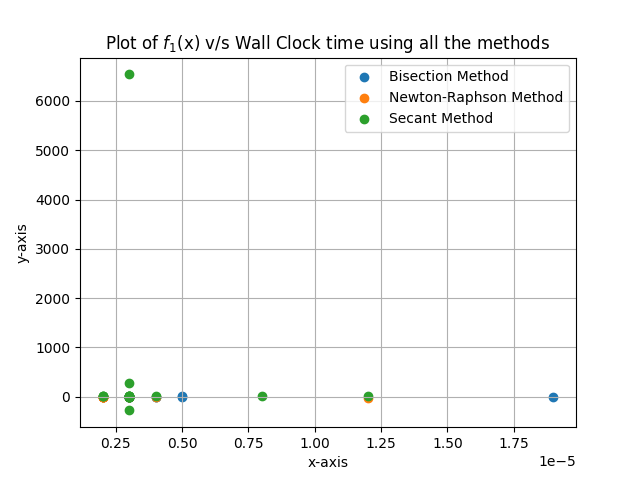
\includegraphics[scale=0.9]{Figure_9.png}
		}
	\end{center}
	\caption{Plot of Metacentric height against Angle of Heel}
\end{figure}
\item The results in this part of the section is based upon the $2^{nd}$ attempt:\\
y = 110 mm.\\
Zero error = 0.5  $^{\circ}$. \\
Theoretical GM = 78.15 mm.\\
From the graph, the value of GM when $\theta = $0  $^{\circ}$ is 44.40 mm.\\
\begin{table}[!ht]
\begin{center}
\begin{tabular}{|p{2cm}|p{2cm}|p{2cm}|p{6cm}|}
\hline
x (mm) & $\theta$ (degree) & tan $\theta$ & Experimental GM (mm) \\
\hline
10 & 3 & 0.0524 & 44.60\\
20 & 5.5 & 0.0963 & 48.54\\
30 & 8.5 & 0.1495 & 46.90\\
40 & 11 & 0.1944 & 48.09\\
45 & 12.5 & 0.2217 & 47.44\\
-10 & -3 & -0.0524 & 44.60\\
-20 & -5 & -0.0875 & 53.42\\
-30 & -8.5 & -0.1495 & 46.90\\
-40 & -11 & -0.1944 & 48.09\\
-45 & -12.5 & -0.2217 & 47.44\\
\hline
\end{tabular}
\end{center}
\end{table}
\newpage
\begin{figure}[!ht]
	\begin{center}
	   \framebox{
			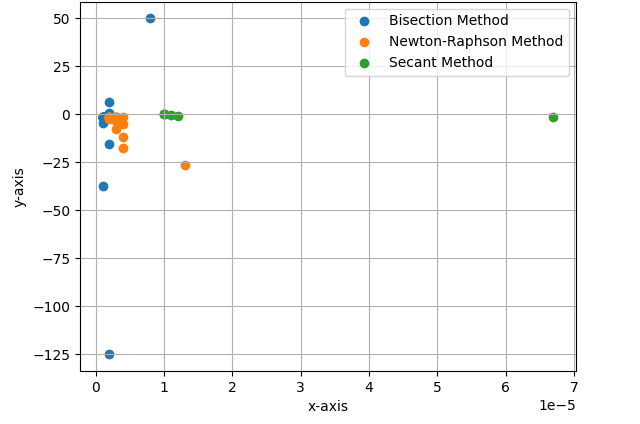
\includegraphics[scale=0.9]{Figure_10.png}
		}
	\end{center}
	\caption{Plot of Metacentric height against Angle of Heel}
\end{figure}
\end{itemize}
\section{Sources of Error:}
From the graphs, we can infer that the theoretically calculated values for metacentric height fairly agree with the experimentally derived values. Error is nearly $=$ 30\%.
The deviations in values could be due to the errors listed below:
\begin{itemize}
\item Error in taking readings.
\item Errors in the apparatus.
\item Low degree of precision.
\item Variations in experimental conditions.
\item Assumptions made to derive the formulae are not strictly satisfied.
\end{itemize}
\section{Conclusion:}
I conclude that the experimentally derived values of metacentric height fairly agree with the theoretically calculated values with some experimental errors. The values of GM at the lowest values of $\theta$ are likely to be less accurate because at smaller
values, minor error in readings cause a greater change in $\frac{\text{1}}{\text{$tan \theta$}}$. The deviations in values can be reduced by greater care in taking readings and the use of more precise instruments.
\end{document}
